% Para documento texto corto
\documentclass[paper=letter,oneside,fontsize=12pt, parskip=full]{article}
%\documentclass[paper=letter,oneside,fontsize=11pt, parskip=full]{scrartcl}
%\documentclass{amsart}
%\documentclass[paper=letter,oneside,fontsize=12pt]{scrartcl}

% Establece dimensiones de los margenes
% \usepackage[inner=1.5cm,outer=3cm,top=2cm,bottom=4cm,
% bindingoffset=5mm]{geometry}
\usepackage[left=2cm,right=2cm,top=3cm,bottom=2cm,
bindingoffset=0cm, footskip=0.5cm, headheight=2cm]{geometry}

% Permite ingresar caracteres acentuados y especiales 
% sin necesidad de emplear comando
% utf8 codificacion de entrada Unicode (mas simbolos que ASCII)
\usepackage[utf8]{inputenc}

% Para usar graficos en archivos externos
\usepackage{graphicx}

% Tabla de tres secciones
\usepackage[flushleft]{threeparttable}

% T1 encoding for European, English, American text
\usepackage[T1]{fontenc}
% Fuente escalable
\usepackage{lmodern}

% Para definir colores
\usepackage{xcolor}
\usepackage{colortbl}

% Para diagramas
\usepackage{smartdiagram}


% Definicion de colores tabla cronograma
\definecolor{colorfa}{rgb}{0.3569,0.608,0.8353}
\definecolor{colorfb}{rgb}{0.4392,0.678,0.2784}
\definecolor{colorfc}{rgb}{1.0000,0.361,0.0000}
\definecolor{colorsem}{rgb}{0.1804,0.455,0.7098}
\definecolor{colorfd}{rgb}{0.9294,0.490,0.1922}
\definecolor{colorfe}{rgb}{0.2667,0.329,0.4157}

% Definicion comandos tabla cronograma
\newcommand{\fa}{\cellcolor{colorfa}}
\newcommand{\fb}{\cellcolor{colorfb}}
\newcommand{\fc}{\cellcolor{colorfc}}
\newcommand{\sem}{\cellcolor{colorsem}}
\newcommand{\fd}{\cellcolor{colorfd}}
\newcommand{\fe}{\cellcolor{colorfe}}

\begin{document}
	
	\section{Propuesta de cambios en TEG}
	
	\subsection{Cambios en diseño del dispositivo Cendit11713}
	
		\begin{figure}[h!] 
			\centering
			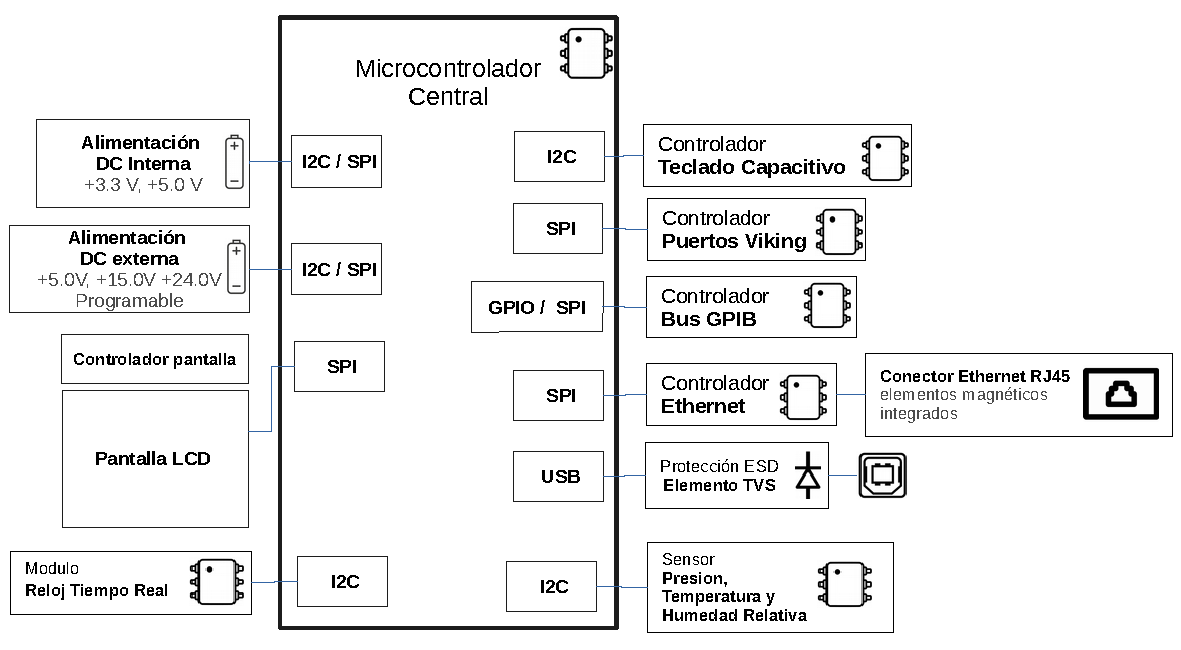
\includegraphics[width=16cm]{Cendit11713BloquesAntes.pdf} \\
			\caption{Propuesta inicial}
		\end{figure}

		\begin{figure}[h!]
			\centering
			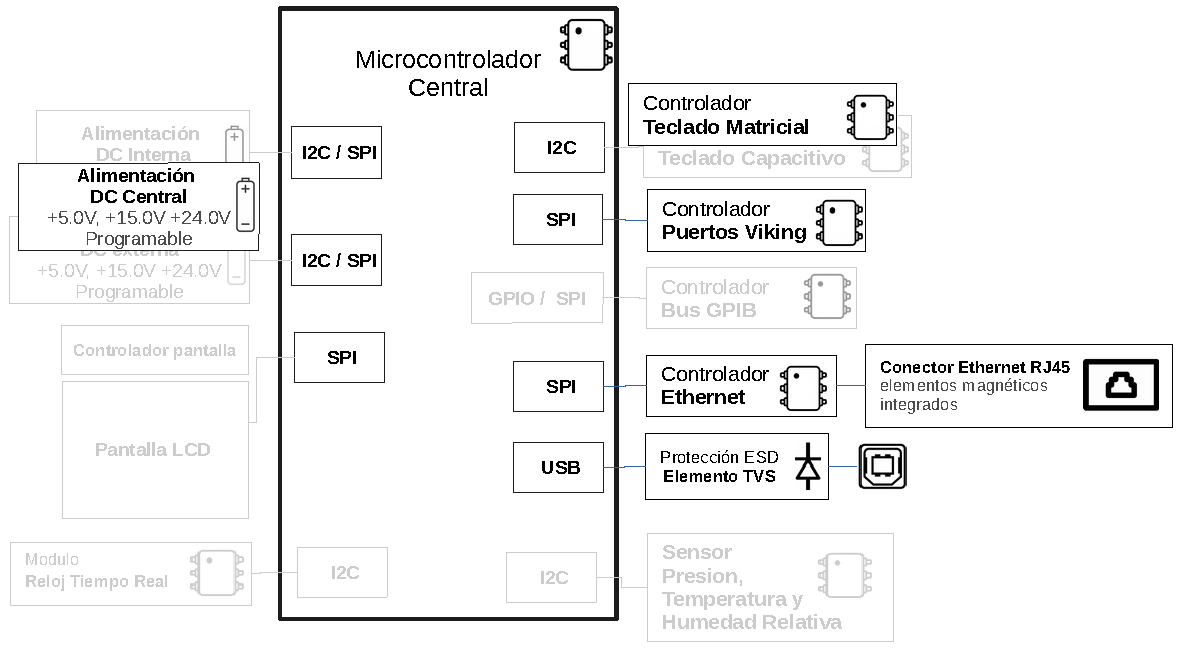
\includegraphics[width=16cm]{Cendit11713BloquesDespues.pdf}
			\caption{Propuesta simplificada}
		\end{figure}	
	
	\subsection{Consideraciones}
	
	El Cendit debe considerar que un proyecto de TEG como el planteado inicialmente es bastante complejo y ambicioso. Implica un proceso de investigación y desarrollo en tres frentes, a saber, hardware, firmware y software. El desarrollo de software y firmware con una calidad aceptable requiere una inversión de tiempo en diseño y depuración que, en etapas iniciales de un proyecto, es difícil de cuantificar. El Cendit debe considerar que es muy difícil generar un producto de calidad bajo la figura de pasante, la asignación salarial sumadas a las adversas condiciones económicas del país dificultan en gran medida el desarrollo de este tipo de proyectos.
	
	También se debe tomar en cuenta la patente falta de interés por parte de la FIUCV en apoyar proyectos de esta envergadura, que permiten adquirir al estudiante un conjunto de conocimientos y destrezas que no son impartidas durante el pregrado.
	
	Durante la fase inicial del proyecto se invirtió una considerable cantidad de tiempo en la documentación bibiográfica sobre el banco de medición de figura de ruido y en la investigación y desarrollo de software para comunicaciones con los instrumentos de este banco. 
	
	Retarde el desarrollo del hardware hasta el momento en logré conseguir la mayor parte de componentes necesarios para el mismo. 
	
	El desarrollo del hardware dependerá en gran medida de la calidad con que se puedan generar las placas de PCB. Hay que tomar en cuenta que se emplea tecnología smd que implica pistas muy finas. Si el método artesanal no da resultados satisfactorios, entoces dependerá del grado de cooperación que brinde el departamento de electrónica del Cendit en la generación de PCBs el desarrollo del hardware.	
		
	Hasta la fecha no he recibid notificación para firmar el addendum del contracto de pasantía.
	
	Para concluir entiendo la necesidad que presenta el Cendit para obtener un diseño que sirva de reemplazo para el controlador de atenuadores e interruptores. Un desarrollo con la robustez y calidad exigidas requiere de su tiempo y esfuerzo para desarrollarse de manera satisfactoria. Tengo gran interes en desarrollar este dispositivos: me peritirá obtener una gran cantidad de conocimientos en el desarrollo de sistemas embebidos.
	
	Pero hay que poner los pies en tierra firme: un proyecto exigente coo el planteado inicialmente definitivamente no puede realizarse bajo la figura de pasante, además me da la impresión que a la FIUCV no le interesa el desarrollo de este tipo de proyectos. Aquí se debe ser pragmático: a la UCV se le dará un desarrollo lo más sencillo posible, no vale la pena invertir esfuerzo y recursos en desarrollar un TEG de este tipo para la UCV, allí nadie tiene interés en este tipo de proyectos!
	
	\subsubsection{Prioridades en diseño de hardware}
	
	\begin{enumerate}
		\item Módulo USB
		\item Módulo puertos Viking
		\item Módulo interfaz de usuario (teclado)
		\item Tarjeta madre
		\item Aplicación de software simplificada
		\item Módulo GPIB (si el tiempo lo permite)
		\item Módulo LAN
	\end{enumerate}

	\subsection{Secuencia de actividades prorroga}
	
	A seguir, de abajo hacia arriba, de la 5 en adelante si el tiempo lo permite.

	\smartdiagram[priority descriptive diagram]{
		1 Desarrollo tarjeta controlador de puertos Viking, 		
		2 Desarrollo tarjeta controlador teclado,
		3 Desarrollo tarjeta madre (en versiones smd y thru hole),
		4 Aplicación CenditLab (versión simplificada),
		5 Desarrollo tarjeta periférico GPIB,
		6 Desarrollo tarjeta periférico LAN			
	}
	
	\subsection{Pautas a seguir en el desarrollo del proyecto}
	
	\begin{enumerate}
	
		\item Una solución de tipo “quick and dirty” para el dispositivo electrónico. Esta es la solución para la UCV. Se realizará una tarjeta madre PCB los más simple posible, tal vez empleando un integrado de tipo thru-hole (no de montaje superficial) en donde reside el micro central acompañado de varios conectores (tiras de pines – pin headers) en cada uno de sus puertos. En estas tiras de pines por medio de cable de cinta se conectará en uno un teclado matricial simple (de 4 x 4), en los otros se conectan las tarjetas expansoras, una de ellas con los transceptores para el bus GPIB.
		
		\item Una aplicación del mismo tipo, “quick and dirty”, únicamente con cuatro pantallas para cada proceso de medición, configuración y calibración para: medición de figura de ruido, medición de potencia de ruido, medición de ganancia, configuración. Esta aplicación es para la UCV. En principio no posee capacidad para corrección por medio de parámetros S de los dispositivos de conexión ni capacidad de simulación. Estas características se agregaran si hay tiempo y una vez completada las tarjetas PCB.	
	
	\end{enumerate}
	
	
	\subsection{Cronograma inicial TEG}
	
		\begin{threeparttable}[!h]
			\centering
			\arrayrulecolor{gray}
			\setlength{\extrarowheight}{4pt}		
			\resizebox{\textwidth}{!}{
				\begin{tabular}{|c|l|l|l|l|l|l|l|l|l|l|l|l|l|l|l|l|l|l|l|l|l|l|l|l|l|l|l|l|}
					\hline 			
					\textbf{Semanas} & 1 & 2 & 3 & 4 & 5 & 6 & 7 & 8 & 9 & 10 & 11 & 12 & 13 & 14 & 15 & 16 & 17 & 18 & 19 & 20 & 21 & 22 & 23 & 24 & 25 & 26 & 27 & 28 \\
					\hline
					\textbf{Fase 1}
					& \fa & \fa & \fa & \fa & \fa & \fa & & & & & & & & & & & & & & & & & & & & & & \\			
					\hline			
					\textbf{Fase 2} & & & & & & & \fb & \fb & \fb & \fb & \fb & \fb & \fb & \fb & \fb & \fb & \fb & & & & & & & & & & & \\
					\hline
					\textbf{Fase 3} & & & & & & & & & & & & & & & & & & \fc & \fc & \fc & \fc & \fc & & & & & & \\	
					\hline		
					\textbf{Seminario} & & & & & & & & & & & & & & \sem & & & & & & & & & & & & & & \\
					\hline
					\textbf{Fase 4} & & & & & & & & & & & & & & & & & & & & & & & \fd & \fd & \fd & \fd &  & \\
					\hline
					\textbf{Fase 5} & & & & & & & & & & & & & & & & & & & & & & & & & & & \fe & \fe \\
					\hline	
				\end{tabular}
			}
			\begin{tablenotes}
				\item {\tiny Fecha de inicio: 6 de Marzo de 2017.} 
				\item {\tiny Jornada de 8 horas diarias, lunes a viernes, de 8:00 AM a 12:00 M y de 1:30 PM a 4:30 PM.}
			\end{tablenotes}
		\end{threeparttable}

	
	\subsection{Contabilidad horaria}
	
		\begin{figure}[h!]
			\centering
			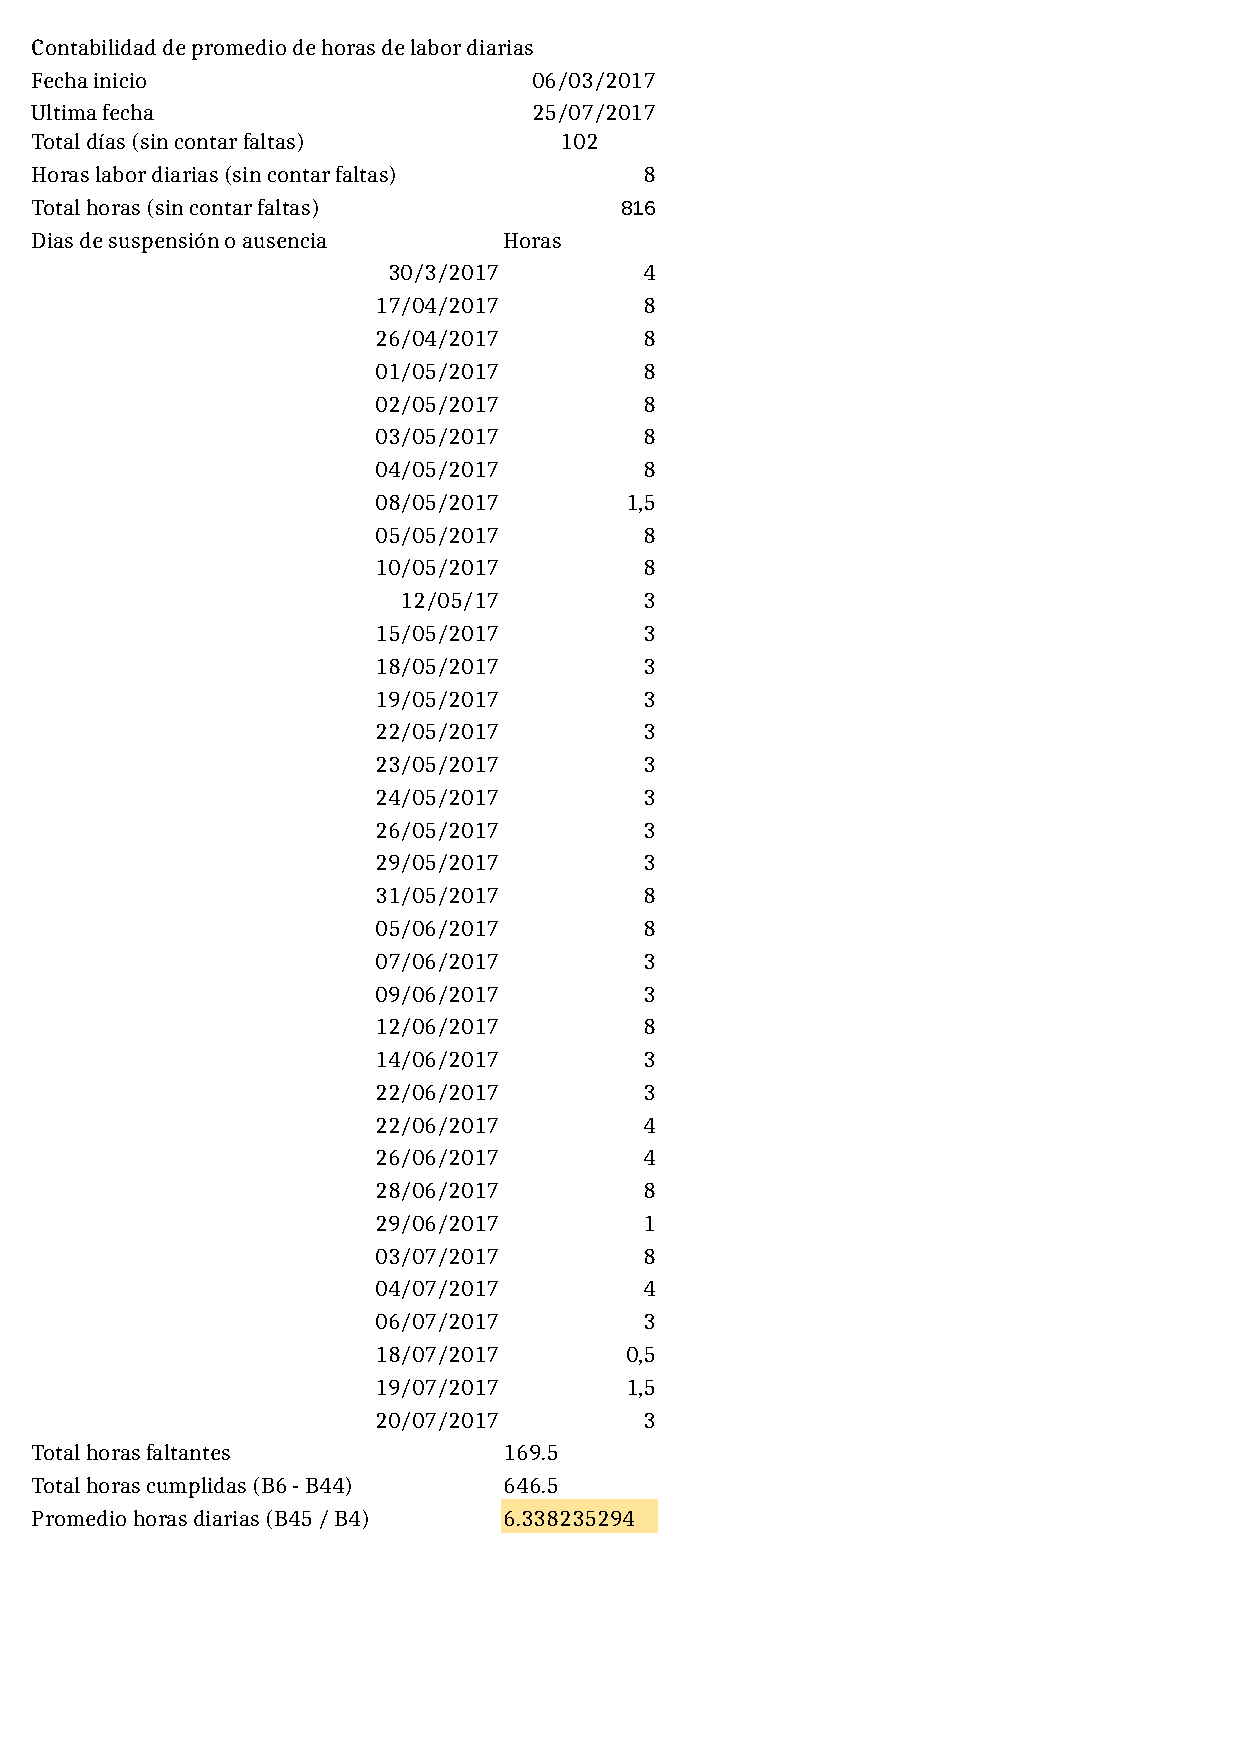
\includegraphics[width=10cm]{ContabilidadHorasPasantia.pdf}
		\end{figure}
	
		Horas totales, disponibles para el TEG: 28 semanas x 7 dias / semana * 8 horas / dia = 1568 horas.
		
		Horas faltantes 169.5 (21 dias). 
		
		Hasta el 25/07/2017 se cumplen 646.5 horas (11.54 semanas). Restarían 921.5 horas (16.45 semanas).		

\end{document}